\setAuthor{Andres Põldaru}
\setRound{lahtine}
\setYear{2019}
\setNumber{G 10}
\setDifficulty{10}
\setTopic{TODO}

\prob{Lame maa}
Juku lendab lennukiga $h=\SI{10}{km}$ kõrgusel, suunab kaamera optilise peatelje horisondile ja teeb pildi. Seejärel trükib ta pildi 10x10 cm paberile ($L=\SI{10}{cm}$). Kui palju on pildi servas horisont maakera kumeruse tõttu madalamal kui pildi keskel? Võib eeldada, et see suurus on väga väike. Kaamera vaatenurk $2\beta=\SI{50}{\degree}$, Maa raadius $R=\SI{6000}{km}$. 



\hint

\solu
Lennukist nähtav maakera horisont moodustab ringjoone. Selle ringjoone eri punktid asuvad kaamerast eri kaugustel. Millise kujutise kaamera sensorile tekitab ringjoon, mille erinevate punktide kaugus kaamerast on erinev?

Kõik kaamera vaatenurgas olevad ringjoone punktid on kaamerast väga kaugel. Kindlasti on lennukist näha kilomeetrite kaugusele, aga kaamera ise on väike. Seega on kõik horisondi punktid sisuliselt lõpmatuses ja võime heas lähenduses eeldada, et kaamera on nendele samaaegselt fokusseeritud. Kujutise leidmiseks tuleb kõik kiired projekteerida suvalisse tasandisse, mis on kaamera optilise peateljega risti.

Teeme joonise nr 1 maakera läbilõikega, kus Juku asub maakera kohal punktis $P$. Kaamera optiline peatelg on suunatud punkti $Q$. Olgu äärmine nähtav horisondi punkt $A$ ja selle projektsioon joonise tasandile $E$. Lennukist nähtava horisondi poolt moodustatud ringjoone keskpunkt on $O$. Projekteerime lennukist (punktist $P$) tõmmatud kiired tasandile, mis on optilise peateljega risti ja läbib punkti $E$.

Joonisel nr 2 on kujutatud horisondi ringjoont keskpunktiga $O$ eraldi, kus on näha äärmine nähtav punkt $A$ ja selle projektsioon $E$ eelmise joonise tasandisse. Heas lähenduses $\angle AOQ = \beta$, sest punktid $O$ ja $P$ on teineteisele lähedal ja pildi peal on punkti $A$ näha pildi servas peaaegu serva keskel (joonis 3). Täpselt pildi keskel on äärmiste punktide vahel $2\beta = \SI{60}{\degree}$.

\begin{center}
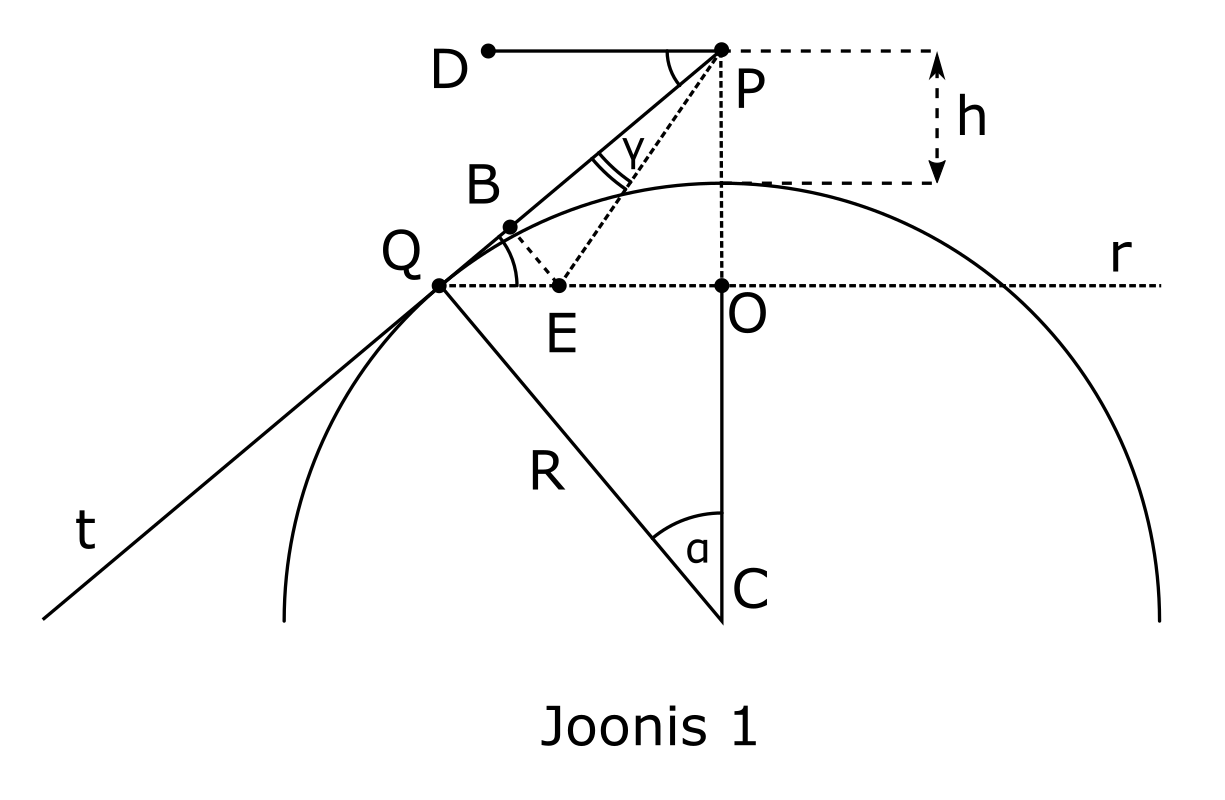
\includegraphics[width=0.50\textwidth]{2019-lahg-10-sol1.png}
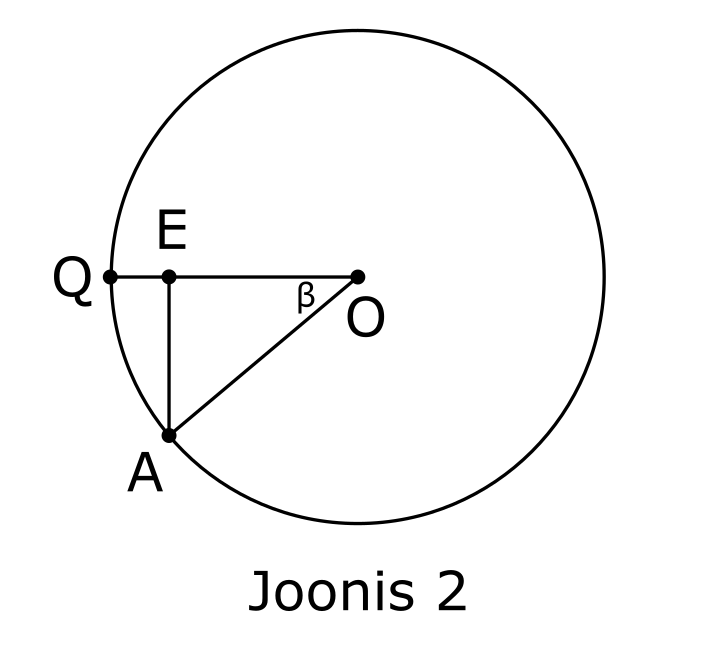
\includegraphics[width=0.265\textwidth]{2019-lahg-10-sol2.png}
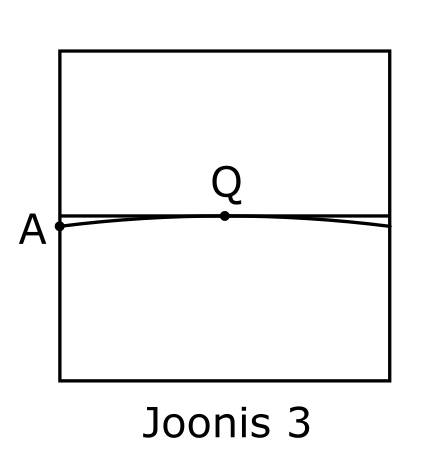
\includegraphics[width=0.215\textwidth]{2019-lahg-10-sol3.png}
\end{center}

Äärmise kiire projektsioon $|BE|$ vastab pildi peal üles-alla suunale. Seda projektsiooni iseloomustab nurk $\gamma=\SI{90}{\degree}-\alpha -\angle EPO$. 
Joonisel 1 leiame $$\cos{\alpha}=\frac{R}{R+h},$$ kust $$\alpha\approx\SI{3.3}{\degree}.$$ Veel leiame $$|OQ|=R\sin{\alpha}\approx \alpha R$$ ja $$|OP|=R+h-R\cos{\alpha}=\frac{h^2+2Rh}{R+h}\approx 2h.$$ Joonise 2 abil leiame $$|OE|=|OQ|\cos{\beta}\approx \alpha R\cos{\beta}.$$

Nüüd saame leida joonisel 1 nurga $\gamma$.
$$\gamma = \SI{90}{\degree}-\alpha-\angle EPO = \SI{90}{\degree}-\alpha-\arctan{\frac{|OE|}{|OP|}}\approx \SI{0.34}{\degree}.$$
Nurgale vastava suuruse pildil saame leida, arvestades, et poolele vaatenurgale $\beta=\SI{25}{\degree}$ vastab $\SI{5}{cm}$. Projektsioonid samasse optilise peateljega ristuvasse tasandisse on võrdelised vastavate projektsioonidega välja prinditud pildil. $$\frac{x}{\SI{5}{cm}}=\frac{\tan{\gamma}}{\tan{\beta}} \rightarrow x = \SI{0.64}{mm}.$$

{\bf Alternatiivne lahendus:} Joonistame vaatluspunktist $P$ maakerale $M$ puutujakoonuse $K$ ning olgu $M$ ja $K$ puutejoon ring $R$ keskpunktiga $O$. Olgu ringil $R$ punkt $Q$ pildivälja keskpunktiks. Tähistame punkti $Q$ läbiva $M$ puutujatasandi $t$-ga ning ringi $R$ poolt defineeritud tasandi $r$-ga. Olgu $r$ ja $t$ lõikejoon $T$. Teoreemist ringi puutujate kohta näeme, et $|PQ|=\sqrt{dh}$, kus $d$ on Maa diameeter ja $h$ - vaatluspunkti kõrgus. Seega nurk, mille all paistab Maa keskpunktist lõik $OQ$ on väikeste nurkade lähenduses $\alpha \approx 2|PQ|/d=2\sqrt{h/d}$ ning $|OP|\approx \alpha |PQ|=2h$. Märgime ringil $r$ punkti $A$ nii, et kaarele $QA$ vastav kesknurk oleks $\beta=25^\circ$; punkti $A$ kujutis asub pildi serval ning sirge $T$ kujutiseks on sirgjoon. Tõmbame punktist $A$ ristsirge tasandile $t$; tähistame selle ristsirge lõikepunkti tasandiga $t$ $B$-ga. Lõigu $AB$ kujutis pildil on meie otsitav suurus. Et punkti $A$ kaugus sirgest $T$ on $|OQ|(1-\cos\beta)$ ja tasandite $t$ ning $r$ vaheline nurk sarnaste kolmnurkade põhjal $\alpha \ll 1$, siis $|AB|\approx \alpha |OQ|(1-\cos\beta)\approx 2h(1-\cos\beta)$. Punkti $A$ kaugus sirgest $PQ$ omab ligikaudu pikkust $a=|OQ|\sin\beta$ ja kujutub pildi poollaiuseks $a'=\SI 5{cm}$.Järelikult kujutub lõik $AB$ lõiguks pikkusega $|AB|a'/a\approx a'\alpha(1-\cos\beta)/\sin\beta\approx 2a'\sqrt{h/d}(1-\cos\beta)/\sin\beta\approx \SI{0.64}{mm}$.
\probend